\documentclass[aspectratio=169, 10pt]{beamer}

\usepackage{bm} % bold math
\usepackage{fontspec}
\usepackage{minted}
\usepackage{pgf-pie}
\usepackage{tikz}
\usepackage{graphicx}
\newcommand\sbullet[1][.5]{\mathbin{\vcenter{\hbox{\scalebox{#1}{$\bullet$}}}}}

% Custom commands and environments
\makeatletter
\newcommand\version[1]{\renewcommand\@version{#1}}
\newcommand\@version{}
\def\insertversion{\@version}

\newcommand\course[1]{\renewcommand\@course{#1}}
\newcommand\@course{}
\def\insertcourse{\@course}

\newcommand\coursetitle[1]{\renewcommand\@coursetitle{#1}}
\newcommand\@coursetitle{}
\def\insertcoursetitle{\@coursetitle}

\newcommand\lecturenumber[1]{\renewcommand\@lecturenumber{#1}}
\newcommand\@lecturenumber{}
\def\insertlecturenumber{\@lecturenumber}
\makeatother

\newcommand{\slidetitle}[1]{{\xbseries \large \structure{#1}} \bigskip}
\newcommand{\term}[1]{{\color{blue} #1}}
\newcommand{\leftspace}{\hspace{1em}}
\newcommand{\inlinearrow}{
  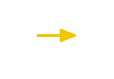
\begin{tikzpicture}[baseline]
    \node [anchor=base] (x) {};
    \draw [rawarrow] (x.mid west) -- ($(x.mid west) + (2em,0)$);
  \end{tikzpicture}
}

\newenvironment{slide}
{\begin{frame}[fragile,environment=slide]\vskip0pt plus 1filll}
{\vskip0pt plus 1filll\end{frame}}

% LaTeX

\setlength{\leftmargini}{1em}

% Common Information

\author{Talia Xu}
\course{COMPSCI 340}
\coursetitle{Operating Systems}
\date{2024 Semester 2}

% fontspec

\defaultfontfeatures{Ligatures=TeX}
% \setmainfont{Domine}
\setsansfont{Inter}[
  FontFace={ul}{n}{Font=*-Thin},
  FontFace={el}{n}{Font=*-ExtraLight},
  FontFace={l}{n}{Font=*-Light},
  FontFace={sb}{n}{Font=*-SemiBold},
  FontFace={eb}{n}{Font=*-ExtraBold},
  FontFace={xb}{n}{Font=*-Black},
]
\setmonofont[Contextuals=AlternateOff, Ligatures=TeXOff]{Iosevka}[
  FontFace={xb}{n}{Font=*-Heavy},
]

%% Font Weights

\DeclareRobustCommand{\ulseries}{\fontseries{ul}\selectfont}
\DeclareTextFontCommand{\textul}{\ulseries}
\DeclareRobustCommand{\elseries}{\fontseries{el}\selectfont}
\DeclareTextFontCommand{\textel}{\elseries}
\DeclareRobustCommand{\lseries}{\fontseries{l}\selectfont}
\DeclareTextFontCommand{\textl}{\lseries}
\DeclareRobustCommand{\sbseries}{\fontseries{sb}\selectfont}
\DeclareTextFontCommand{\textsb}{\sbseries}
\DeclareRobustCommand{\ebseries}{\fontseries{eb}\selectfont}
\DeclareTextFontCommand{\texteb}{\ebseries}
\DeclareRobustCommand{\xbseries}{\fontseries{xb}\selectfont}
\DeclareTextFontCommand{\textxb}{\xbseries}

% tikz

\usetikzlibrary{
  arrows,
  arrows.meta,
  automata,
  backgrounds,
  calc,
  decorations.pathreplacing,
  matrix,
  positioning,
  overlay-beamer-styles,
  shapes,
  shapes.multipart,
  tikzmark,
}

\tikzstyle{rawarrow} = [
  -{Latex[round]},
  line width=1pt,
  yellow,
  shorten >=3pt,
  shorten <=3pt,
  font=\small,
  text=black,
]

\tikzstyle{arrow} = [
  -{Latex[round]},
  line width=1pt,
  yellow,
  shorten >=3pt,
  shorten <=3pt,
  transform canvas={yshift=3pt},
  font=\small,
  text=black,
]

\newcommand{\tikzmarkcoord}[1]{([yshift=3pt]pic cs:#1)}

% minted

\setminted{style=eyolfson, fontsize=\small, escapeinside=||}
\setmintedinline{fontsize=\normalsize}

% hyperref

\hypersetup{colorlinks, urlcolor=blue}

% beamer
\setbeamersize{text margin left=16mm, text margin right=16mm}
\setbeamertemplate{itemize items}[circle]
\setbeamercolor{item}{fg=black}
\setbeamercolor{structure}{fg=darkblue}
\setbeamerfont{frametitle}{series=\bfseries, parent=structure}
\setbeamertemplate{navigation symbols}{}
\setbeamertemplate{headline}{}
\setbeamertemplate{footline}{
  \begin{tikzpicture}[
    remember picture,
    overlay,
    shift={(current page.south west)},
  ]
    \path [fill=gray] (144mm, 0) -- (160mm, 16mm) -- (160mm, 0);
    \node [inner sep=3.5mm, outer sep=0, text=black, anchor=base east,
           align=right, yshift=3.5mm]
          at (current page.south east) {\ttfamily \small \insertframenumber{}};
  \end{tikzpicture}
}
\setbeamertemplate{title page}{
  \begin{tikzpicture}[
    remember picture,
    overlay,
    shift={(current page.south west)},
    background rectangle/.style={fill=darkblue},
    show background rectangle,
  ]
    \node [anchor=center, align=center, text=white, text width=40mm, scale=3.2]
          at (\paperwidth / 2, \paperheight * 2 / 3)
          {\xbseries \inserttitle{}};
    \node [anchor=base west, align=left, inner sep=0, text=white, yshift=2.5mm]
          at (16mm, \paperheight / 3)
          {\insertdate{} \insertcourse{}: \insertcoursetitle{}};
    \node [anchor=base west, align=left, inner sep=0, text=white, yshift=-2.5mm]
          at (16mm, \paperheight / 3)
          {\insertauthor};
    \node [anchor=base east, align=right, inner sep=0, text=white, yshift=2.5mm]
          at (144mm, \paperheight / 3)
          {Lecture \insertlecturenumber{}};
    \node [anchor=base east, align=right, inner sep=0, text=white,
           yshift=-2.5mm]
          at (144mm, \paperheight / 3)
          {\ttfamily \insertversion{}};
    \node [align=center, anchor=south, inner sep=0, text=white, yshift=3.5mm]
          (license) at (\paperwidth / 2, 0)
          {\fontsize{7pt}{7pt}\selectfont This  work is licensed under a
           \href{http://creativecommons.org/licenses/by-sa/4.0/}
                {\color{lightblue} Creative Commons Attribution-ShareAlike 4.0
                 International License}};
  \end{tikzpicture}
}

% xcolor

%% Primary Colour

\definecolor{pantone655}{RGB}{0, 42, 92} % #002a5c
\colorlet{darkblue}{pantone655}

%% Secondary Colours

\definecolor{pantone633}{RGB}{0, 139, 176} % #008bb0
\colorlet{blue}{pantone633}

\definecolor{pantonewarmred}{RGB}{220, 70, 51} % #dc4633
\colorlet{red}{pantonewarmred}

\definecolor{pantone3285}{RGB}{0, 161, 137} % #00a189
\colorlet{cyan}{pantone3285}

\definecolor{pantone7722}{RGB}{13, 83, 77} % #0d534d
\colorlet{darkcyan}{pantone7722}

\definecolor{pantone376}{RGB}{141, 191, 46} % #8dbf2e
\colorlet{green}{pantone376}

\definecolor{pantone2613}{RGB}{109, 36, 122} % #6d247a
\colorlet{violet}{pantone2613}

\definecolor{pantone2985}{RGB}{111, 199, 234} % #6fc7ea
\colorlet{lightblue}{pantone2985}

\definecolor{pantone227}{RGB}{171, 19, 104} % #ab1368
\colorlet{magenta}{pantone227}

\definecolor{pantone7406}{RGB}{241, 197, 0} % #f1c500
\colorlet{yellow}{pantone7406}

%% Neutrals

\definecolor{pantonecoolgray2}{RGB}{208, 209, 201} % #d0d1c9
\colorlet{gray}{pantonecoolgray2}


\lecturenumber{1}
\title{File\\Systems}
\version{1.0.0}
 
\begin{document}

\begin{frame}[plain, noframenumbering]
    \titlepage
\end{frame}

\begin{slide}
	
	\slidetitle{Inter-computer communication}
	
	Without shared memory, computers need a network to communicate.
	\bigskip
	
	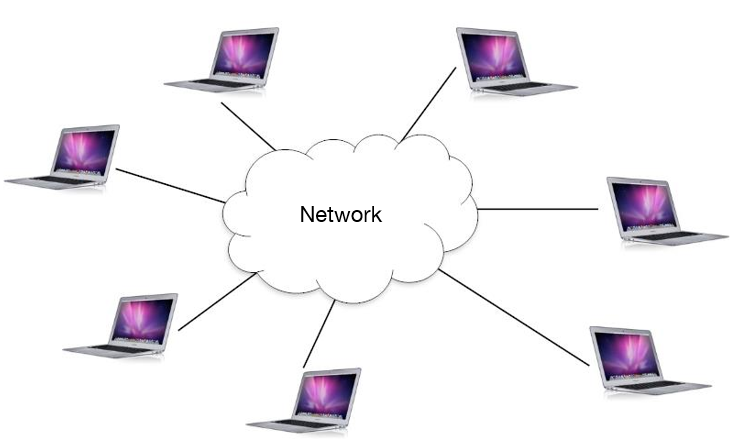
\includegraphics[width=80mm]{inter-computer-comm.png}
	
\end{slide}

\begin{slide}

	\slidetitle{Modes of connection: two design approaches}
	
	Circuit switching (virtual circuit)
	\begin{itemize}
		\item Dedicated path (route) established at setup
		\item Guaranteed (fixed) bandwidth - routers commit to resources
		\item Typically fixed-length packets (cells), each cell only need a virtual circuit ID
		\item Constant latency
	\end{itemize}
	\bigskip
	
	Packet switching (datagram)
	\begin{itemize}
		\item Shared connection; competition for use with others
		\item Data is broken into chunks called packets
		\item Each packet contains a desitnation address
		\item Available bandwidth is up to channel capacity (often smaller)
		\item Variable latency
	\end{itemize}

\end{slide}

\begin{slide}

	\slidetitle{Network protocol layering}
	
	Most popular model of guiding (not specifying) ptotocol layrs is the OSI reference model.
	\medskip
	
	\begin{minipage}{0.3\textwidth}
	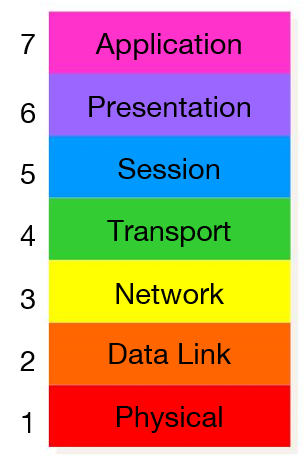
\includegraphics[width=35mm]{OSI-model.png}
	\end{minipage}
	\hfill
	\begin{minipage}{0.68\textwidth}
		7. Application: HTTP, email, FTP
		\medskip
		\smallskip
		
		6. Presentation: XDR, MIME, JSON, XML
		\medskip
		\smallskip
		
		5. Session: HTTP 1.1, SSL
		\medskip
		\smallskip
		
		4. Transport: TCP, UDP
		\medskip
		\smallskip
		
		3. Network: IP, X.25
		\medskip
		\smallskip
		
		2. Data Link: Ethernet MAC, PPP
		\medskip
		\smallskip
		
		1. Physical: USB, Bluetooth, Wi-Fi radios
	\end{minipage}

\end{slide}

\begin{slide}

	\slidetitle{Protocol Encapsulation}
	
	At any layer:
	\begin{itemize}
		\item The higher-level protocol headers are just treated like data
		\item Lower-level protocol headers can be ignored
	\end{itemize}
	
	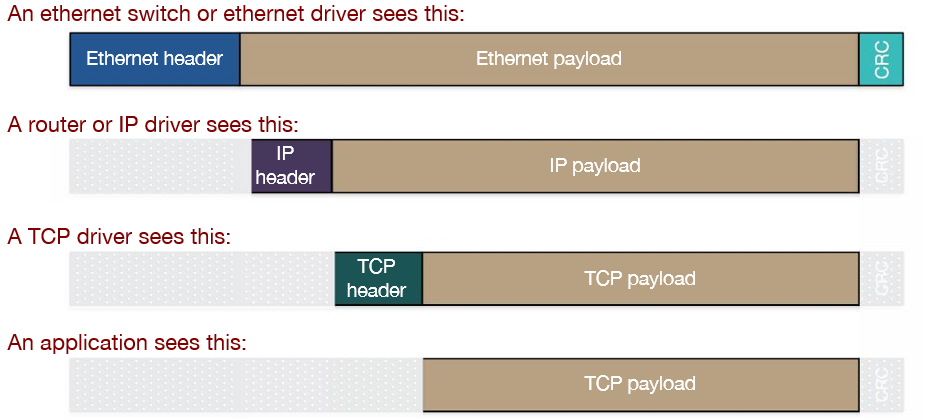
\includegraphics[width=100mm]{protocol-encapsulation.png}
	
\end{slide}

\begin{slide}

	\slidetitle{IP Addressing}
	
	Each network endpoint has a unique IP address
	\begin{itemize}
		\item No relation to an ethernet address
		\item IPv4: 32-bit address
			\begin{itemize}
				\item uoa.auckland.ac.nz = 130.216.5.170
			\end{itemize}
		\item IPv6: 128-bit address
			\begin{itemize}
				\item www.google.com = 2404:6800:4006:804::2004
			\end{itemize}
	\end{itemize}
	\bigskip
	
	Data is broken into packets. Each packet contains
	\begin{itemize}
		\item source and destination IP addresses
		\item Header checksum
		\item Data
	\end{itemize}

\end{slide}

\begin{slide}

	\slidetitle{Communication over IP}
	
	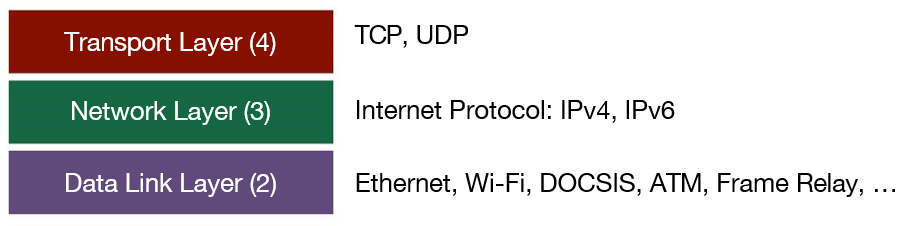
\includegraphics[width=100mm]{comm-over-ip.png}
	\bigskip
	
	TCP: Reliable, in-order byte stream
	\bigskip
	
	UDP: Unreliable, message stream (order not guarantedd)
	
\end{slide}

\begin{slide}

	\slidetitle{Transport Layer}
	
	We want to communicate between applications
	\bigskip
	
	The transport layger gives us logical "channels" for communication
	\begin{itemize}
		\item Processes can write to and receive from these channels.
	\end{itemize}
	\bigskip
	
	Two transport layer protocols in IP are TCP and UDP
	\begin{itemize}
		\item A port number identifies a unique channel on each computer
	\end{itemize}

\end{slide}

\begin{slide}

    \slidetitle{UDP}
	
	All traffic goes to a socket that reads from a host address and port.
	\bigskip
	
	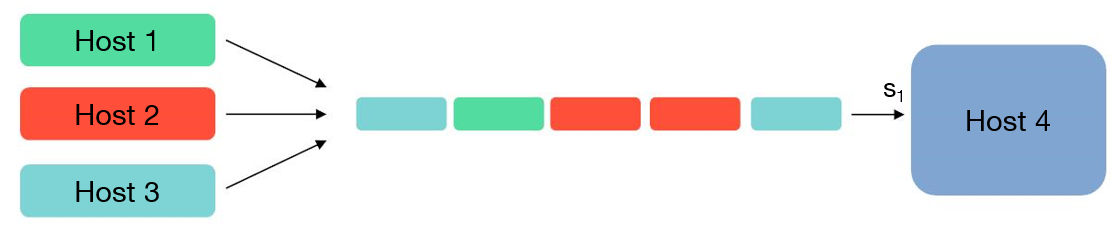
\includegraphics[width=110mm]{udp.png}
	\bigskip
	
	A server creates a socket to receive messages on a specific port number. 
	\bigskip
	
	Packets sent from different processes and/or systems all arrive on the same socket on the server.
	
\end{slide}

\begin{slide}

    \slidetitle{TCP}

	Unique channels identified by
	\begin{itemize}
		\item {Remote host, Remote port, Local host, Local port}
		\item One socket for listening for new connections on a local host, port
		\item Separate communication socket for each "connection"
	\end{itemize}
	\bigskip
	
    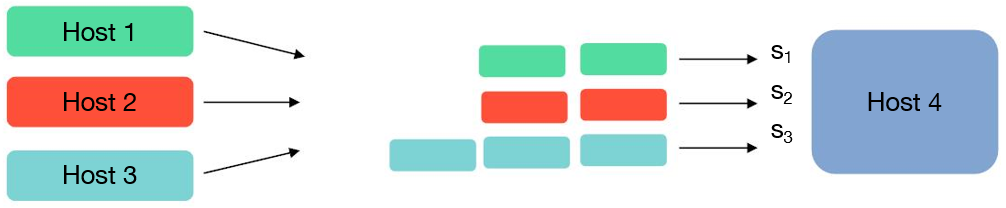
\includegraphics[width=100mm]{tcp.png}
	\bigskip
	
	A server creates a socket to listen for connections on a specific port number.
	\bigskip
	
	Each connection results in a new socket at the server.

\end{slide}

\begin{slide}

	\slidetitle{UDP or TCP?}
	
	\begin{itemize}
		\item Web Browsing
		\item Online Gaming
		\item File Transfer
		\item Zoom
		\item Video Streaming
		\item Music Streaming
	\end{itemize}
	
\end{slide}

\begin{slide}

	\slidetitle{Protocols}
	
	Set of rules (\& customs) for communicating
	\bigskip
	
	Exist at different levels:
	\begin{itemize}
		\item Exist at each layer of the network stack
		\item Meaning of bytes
		\item Sequence of request \& response messages
	\end{itemize}

\end{slide}

\begin{slide}

	\slidetitle{Software interaction model}
	
	Socket API: all we get from the OS to access the network
	\bigskip
	
	Socket = distinct end-to-end communication channels
	\bigskip
	
	Line-oriented, text-based protocols common
	\begin{itemize}
		\item Not efficient but easy to debug and use
	\end{itemize}

\end{slide}

\begin{slide}

	\slidetitle{Problems with the socket APIs}
	
	The sockets interface forces a read/write mechanism
	\bigskip
	
	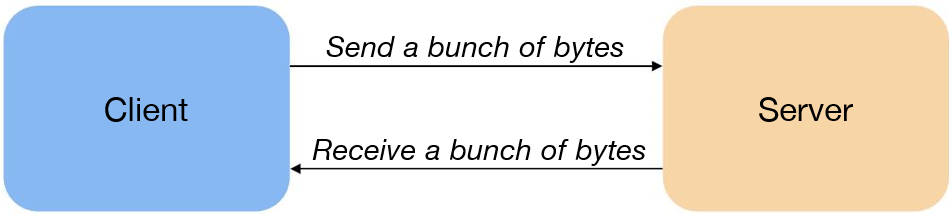
\includegraphics[width=100mm]{socket-api-problem.png}
	\bigskip
	
	Programming is often easier with a functional interface
	\bigskip
	
	To make distributed computing look more like centralized computing, I/O (read/write) is not the way to go.
	
\end{slide}
    
\begin{slide}

    \slidetitle{Remote service - stateful}

    Server knows:
    \begin{itemize}
        \item who has the file open
        \item for what type of access
        \item and where it is in the file etc.
        \item When the client calls open, it receives an identifier to be used to access the file.
        \item Looks very similar to traditional local file access to the client process.
        \item Efficient, the needed data may be read ahead by the server.
        \item Information about the file is held in memory.
        \item If the server crashes
        \begin{itemize}
            \item it is difficult to start again since all the state information is lost.
        \end{itemize}
        \item Server has problems with processes which die
        \begin{itemize}
            \item needs to occasionally check.
        \end{itemize}
    \end{itemize}

\end{slide}

\begin{slide}

    \slidetitle{Remote service - stateless}

    Server does not maintain information on the state of the system. It merely responds to requests.
    \bigskip

    Open and close calls don’t send messages to the server. Handled locally. (Except for access privileges.)
    \bigskip

    Requesting processor has topass all the extra information with each read/write
    \begin{itemize}
        \item e.g., the current file location the process is reading from, accesibility
    \end{itemize}
    \bigskip

    Server doesn't have to worry about processes stopping
    \bigskip

    No complicated recovery process if the server goes down
    
\end{slide}

\begin{slide}

    \slidetitle{Remote Procedue Calls (RPC)}

    RPC abstract attempts to make remote procedure calls look like local ones.

\end{slide}

\begin{slide}

    \slidetitle{Sending a remote call}

    \inputminted[fontsize=\scriptsize]{c}{wmsg.c}

\end{slide}

\begin{slide}

	\slidetitle{Implementing RPC}
	
	No architectural support for remote procedure calls.
	\bigskip
	
	Simulate it with tools we have (local procedure calls)
	\bigskip
	
	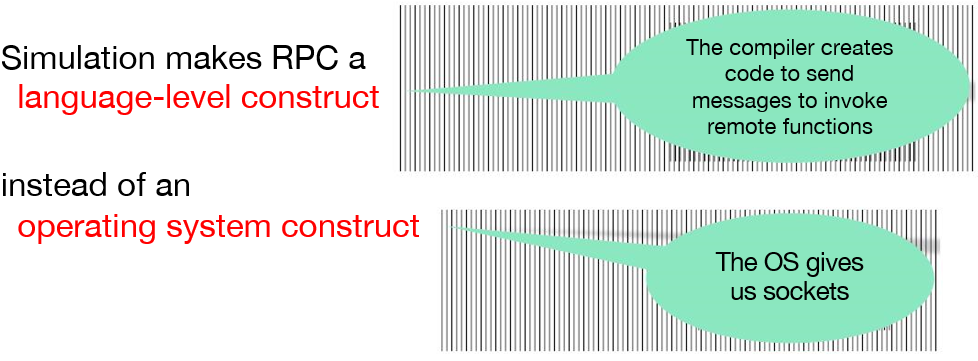
\includegraphics[width=120mm]{implement-rpc.png}

\end{slide}

\begin{slide}

    \slidetitle{Implementing RPC}

    Create stub functions:
	\begin{itemize}
		\item to make it appear to the user that the call is local
	\end{itemize}
	\bigskip
	
	On the clinet:
	\begin{itemize}
		\item The stub function (proxy) has the function’s interface
		\item Packages parameters and calls the server
	\end{itemize}
	\bigskip
	
	On the server:
	\begin{itemize}
		\item The stub function (skeleton) receives the request and calls the local function
	\end{itemize}

\end{slide}

\begin{slide}

	\slidetitle{Interface Definition Language (IDL)}
	
	Allow programmer to specify remote procedure interfaces
	\begin{itemize}
		\item (names, parameters, return values)
	\end{itemize}

	An IDL looks similar to function prototypes.
	
\end{slide}

\begin{slide}

    \slidetitle{Interface definition language (IDL) of an adder}

    \inputminted{python}{Adder.idl}

\end{slide}

\begin{slide}

    \slidetitle{Server and client code with RPC}

    \inputminted{python}{server.py}
    \bigskip

    \inputminted{python}{client.py}

\end{slide}

\begin{slide}

    \slidetitle{Stub generator}
    
    \textbf{Marshalling/Unmarshalling}: Converting data structures into byte streams for transmission (marshalling) and reconstructing them on the receiving end (unmarshalling).
    \bigskip

    \textbf{Buffering}: Temporarily storing data in memory to optimize transmission.
    \bigskip

    \textbf{Message Transmission}: Sending and receiving messages over the network.
    \bigskip

    Server and client code can focus solely on implementing the core application logic.

\end{slide}

\begin{slide}

	\slidetitle{RPC Benefits}

	RPC gives us a procedure call interface
	\bigskip
	
	Writing applications is simplified
	\begin{itemize}
		\item RPC hides all network code into stub functions
		\item Application programmers don't have to worry about details
		\begin{itemize}
			\item Sockets, port numbers, byte ordering
		\end{itemize}
	\end{itemize}
	
\end{slide}

\end{document}
